\documentclass[12pt, twoside]{book}
\usepackage[a4paper,top=2.5cm,bottom=2.5cm,left=3.5cm,right=2cm]{geometry}
\usepackage[utf8]{inputenc}
\usepackage[T1]{fontenc}
\usepackage{graphicx}
\usepackage{url}
\usepackage[hidelinks,breaklinks]{hyperref}
\usepackage[dvipsnames]{xcolor}
\usepackage{mathtools}
\usepackage{amssymb}
\usepackage[slovak]{babel}
\usepackage{lmodern}
\usepackage{algorithm}
\usepackage[noend]{algpseudocode}
\linespread{1.25}

\makeatletter
\renewcommand{\ALG@name}{Algoritmus}
\makeatother

% -------------------
% --- Definicia zakladnych pojmov
% --- Vyplnte podla vasho zadania
% -------------------
\def\mfrok{2019}
\def\mfnazov{Analýza odolnosti Stellar konsenzus protokolu voči Byzantínskym chybám}
\def\mftyp{Bakalárska práca}
\def\mfautor{Samuel Sládek}
\def\mfskolitel{RNDr. Tomáš Kulich, PhD.}

\def\mfmiesto{Bratislava, \mfrok}

%aj cislo odboru je povinne a je podla studijneho odboru autora prace
\def\mfodbor{2508 Informatika} 
\def\program{ Informatika }
\def\mfpracovisko{ Katedra informatiky }

\begin{document}     
\frontmatter


% -------------------
% --- Obalka ------
% -------------------
\thispagestyle{empty}

\begin{center}
\sc\large
Univerzita Komenského v Bratislave\\
Fakulta matematiky, fyziky a informatiky

\vfill

{\LARGE\mfnazov}\\
\mftyp
\end{center}

\vfill

{\sc\large 
\noindent \mfrok\\
\mfautor
}

\eject % EOP i
% --- koniec obalky ----

% -------------------
% --- Titulný list
% -------------------

\thispagestyle{empty}
\noindent

\begin{center}
\sc  
\large
Univerzita Komenského v Bratislave\\
Fakulta matematiky, fyziky a informatiky

\vfill

{\LARGE\mfnazov}\\
\mftyp
\end{center}

\vfill

\noindent
\begin{tabular}{ll}
Študijný program: & \program \\
Študijný odbor: & \mfodbor \\
Školiace pracovisko: & \mfpracovisko \\
Školiteľ: & \mfskolitel \\
% Konzultant: & \mfkonzultant \\
\end{tabular}

\vfill


\noindent \mfmiesto\\
\mfautor

\eject % EOP i


% --- Koniec titulnej strany


% -------------------
% --- Zadanie z AIS
% -------------------
% v tlačenej verzii s podpismi zainteresovaných osôb.
% v elektronickej verzii sa zverejňuje zadanie bez podpisov

\newpage
\thispagestyle{empty}
\hspace{-2cm}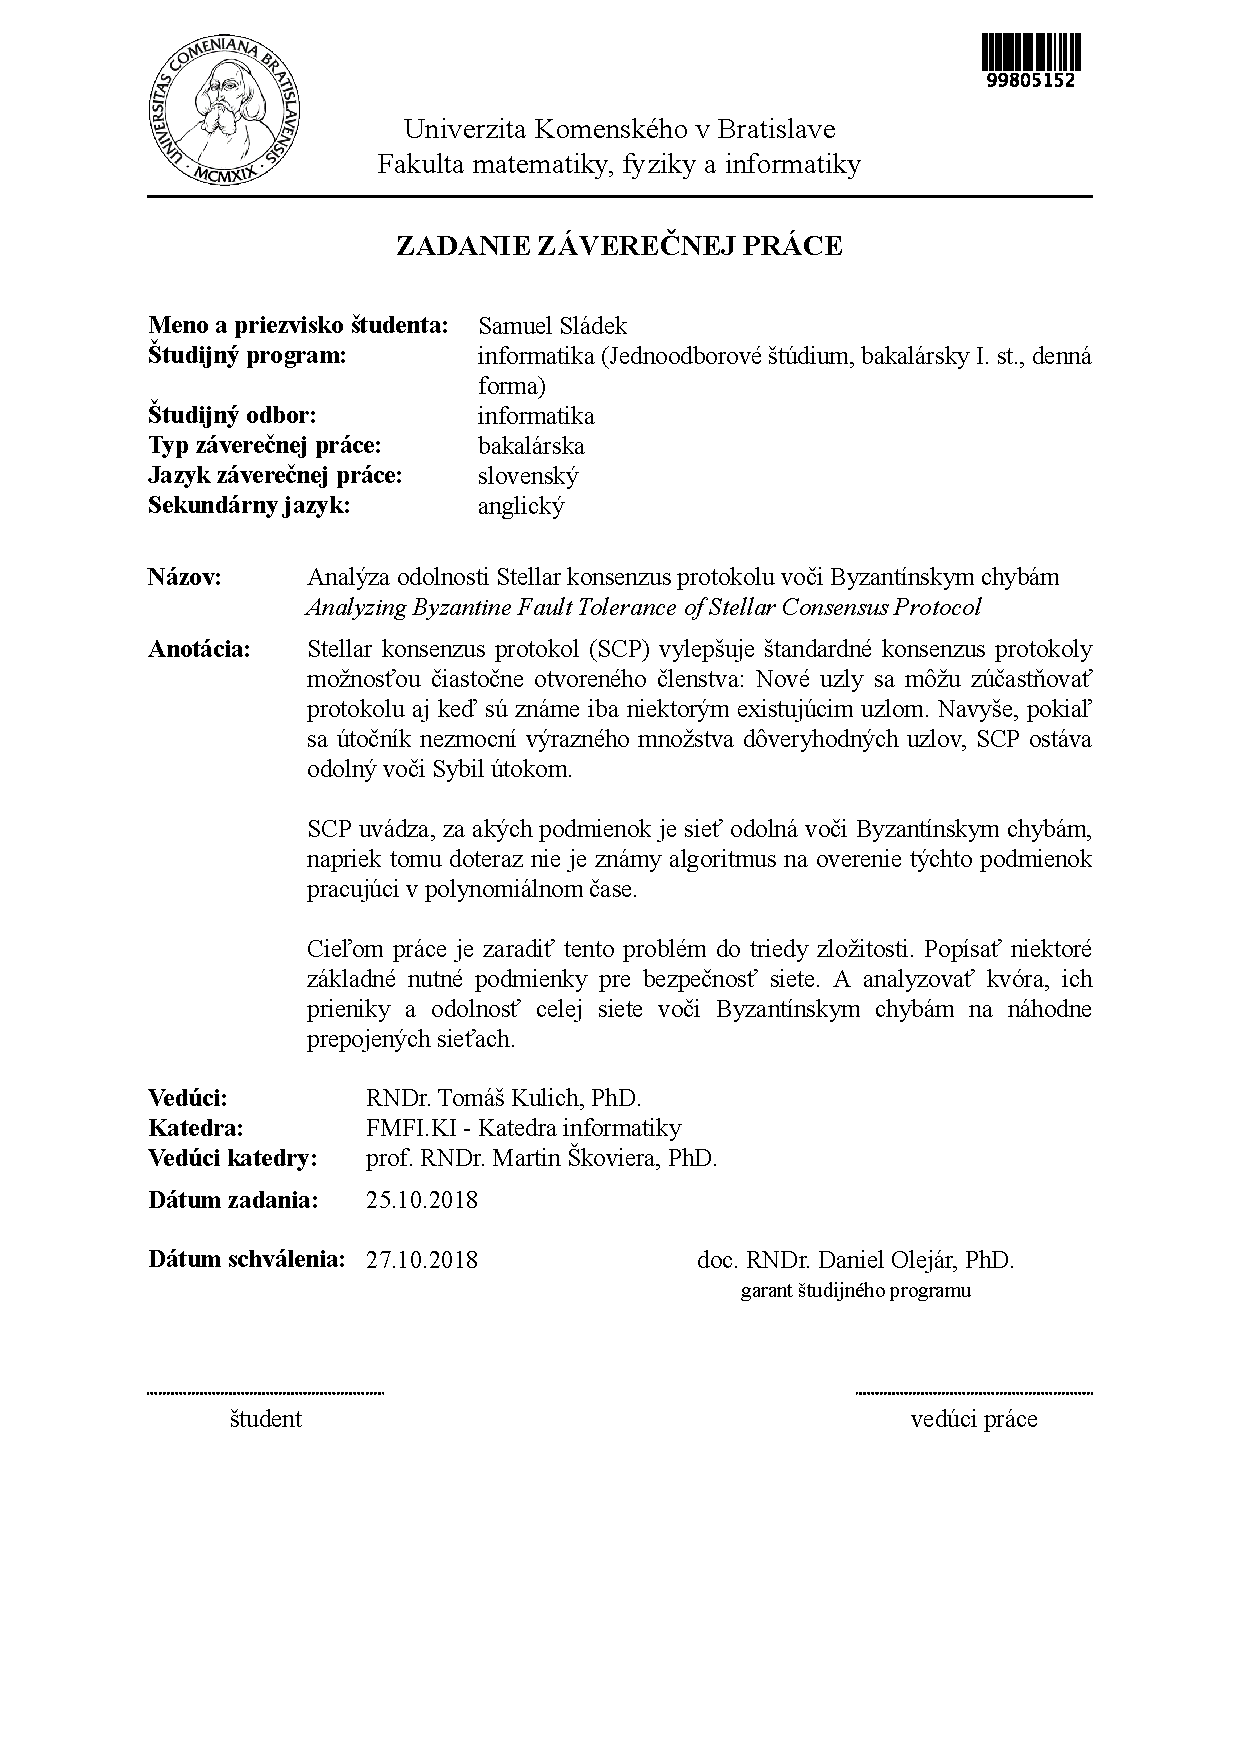
\includegraphics[width=1.1\textwidth]{images/zadanie}

% --- Koniec zadania

\frontmatter

% -------------------
%   Poďakovanie - nepovinné
% -------------------
\setcounter{page}{5}
\newpage

\begin{flushleft}\textbf{\Large Poďakovanie}\end{flushleft}
Chcel by som sa poďakovať môjmu školiteľovi RNDr. Tomášovi Kulichovi, PhD.
za návrh témy a podpory v objavovaní pre mňa nového sveta kryptomien.

Rovnako Patrikovi Bakovi za skvelé rady, postrehy a najmä možnosti
vyrozprávania sa o nástrahách čakajúcich v priebehu vyhotovovania práce.

% --- Koniec poďakovania

% -------------------
%   Abstrakt - Slovensky
% -------------------
\newpage 
\section*{Abstrakt}

Kryptomena Stellar pred pár rokmi prešla na nový protokol, ktorý má vylepšovať
dovtedy známe konsenzus protokoly najmä zjednodušením možnosti vstupu do siete
pre novú entitu.
Táto práca analyzuje odolnosť tohto protokolu voči zlyhaniam jednotlivých
entít spolupracujúcich na konsenze. Najprv ukáže, že pre danú sieť nevieme
v polynomiálnom čase povedať pri koľkých zlyhaniach bude sieť stále bezpečná
a ani pri koľkých zlyhaniach bude sieť stále schopná dohodnúť sa na konsenze.
Neskôr sa pozrie na niektoré zaujímavé typy sietí pri ktorých vieme vyjadriť
odolnosť rýchlo.
Vytvorí tiež algoritmus na presné vyjadrenie odolnosti malých sietí a aj rýchlejší
algoritmus na odhady zhora pre odolnosť väčších sietí.
Na záver rozanalyzuje bezpečnosť a odolnosť náhodne vytvorených sietí.
Túto analýzu ukončí odporúčaním volenia parametrov siete aby bola sieť schopná
prežiť čo najviac zlyhaní.

\paragraph*{Kľúčové slová:} Stellar, konsenzus, byzantínske chyby,
kvórum, bezpečnosť, odolnosť siete
% --- Koniec Abstrakt - Slovensky


% -------------------
% --- Abstrakt - Anglicky 
% -------------------
\newpage 
\section*{Abstract}

A few years ago, cryptocurrency Stellar switched to a new protocol
to improve previously known consensus protocols in particular by simplifying
network entry for a new entity.
This thesis analyzes the resilience of this protocol to Byzantine failures.
Firstly it shows impossibility to evaluate number of failures in which the
network is still safe and the number of failures in which the network can still
agree on consensus in polynomial time.
Later, it considers some interesting types of networks in which we are able
to calculate resilience quickly.
It creates algorithm to accurately express resilience for small networks and
faster one to determine the upper bound for resilience of larger networks.
At the end it analyzes security and resilience of randomly created networks.
This analysis ends with recommendations for choosing network parameters to
make resilience as high as possible.



\paragraph*{Keywords:}  Stellar, consensus, Byzantine failures,
quorum, safety, network resilience

% --- Koniec Abstrakt - Anglicky

% -------------------
% --- Predhovor - v informatike sa zvacsa nepouziva
% -------------------
%\newpage 
%\thispagestyle{empty}
%
%\huge{Predhovor}
%\normalsize
%\newline
%Predhovor je všeobecná informácia o práci, obsahuje hlavnú charakteristiku práce 
%a okolnosti jej vzniku. Autor zdôvodní výber témy, stručne informuje o cieľoch 
%a význame práce, spomenie domáci a zahraničný kontext, komu je práca určená, 
%použité metódy, stav poznania; autor stručne charakterizuje svoj prístup a svoje 
%hľadisko. 
%
% --- Koniec Predhovor


% -------------------
% --- Obsah
% -------------------

\newpage 

\tableofcontents

% ---  Koniec Obsahu

% -------------------
% --- Zoznamy tabuliek, obrázkov - nepovinne
% -------------------

\newpage 

\listoffigures
%\listoftables

% ---  Koniec Zoznamov

\mainmatter


\input uvod.tex 

\input consenzus.tex

\input stellar.tex

\input security.tex

\input particular_networks.tex

\input random.tex

\input zaver.tex

% -------------------
% --- Bibliografia
% -------------------


\newpage	

\backmatter

\thispagestyle{empty}
\nocite{*}
\clearpage

\addcontentsline{toc}{chapter}{Literatúra} % rucne pridanie do obsahu
\bibliographystyle{plain}
\bibliography{literatura}

%Prípadne môžete napísať literatúru priamo tu
%\begin{thebibliography}{5}
 
%\bibitem{br1} MOLINA H. G. - ULLMAN J. D. - WIDOM J., 2002, Database Systems, Upper Saddle River : Prentice-Hall, 2002, 1119 s., Pearson International edition, 0-13-098043-9

%\bibitem{br2} MOLINA H. G. - ULLMAN J. D. - WIDOM J., 2000 , Databasse System implementation, New Jersey : Prentice-Hall, 2000, 653s., ???

%\bibitem{br3} ULLMAN J. D. - WIDOM J., 1997, A First Course in Database Systems, New Jersey : Prentice-Hall, 1997, 470s., 

%\bibitem{br4} PREFUSE, 2007, The Prefuse visualization toolkit,  [online] Dostupné na internete: <http://prefuse.org/>

%\bibitem{br5} PREFUSE Forum, Sourceforge - Prefuse Forum,  [online] Dostupné na internete: <http://sourceforge.net/projects/prefuse/>

%\end{thebibliography}

%---koniec Referencii

% -------------------
%--- Prilohy---
% -------------------

\input attachments.tex

%\addcontentsline{toc}{chapter}{Appendix A}
%\input AppendixA.tex
%
%\addcontentsline{toc}{chapter}{Appendix B}
%\input AppendixB.tex

\end{document}






